\documentclass[11pt,a4paper]{article}
\usepackage[T1]{fontenc}
\usepackage[utf8]{inputenc}
\usepackage{lmodern}
\usepackage{textcomp}
\usepackage[left=1.8cm,right=1.8cm,top=3.0cm,bottom=2.2cm,headheight=36pt,headsep=12pt]{geometry}
\usepackage{multicol}
\usepackage{xcolor}
\usepackage{fancyhdr}\usepackage{tikz}
\usepackage{graphicx}
\usepackage{array}
\usepackage{amsmath,amssymb}
\usepackage{setspace}
\usepackage{longtable}
\graphicspath{{../}}
\definecolor{ygreen}{RGB}{46,139,87}\definecolor{dgreen}{RGB}{28,90,56}
\renewcommand{\normalsize}{\fontsize{10.9}{13.4}\selectfont}
\renewcommand{\familydefault}{\rmdefault}
\setlength{\parindent}{0pt}
\setlength{\columnsep}{0.8cm}
\setlength{\columnseprule}{0.4pt}
\setlength{\multicolsep}{3pt plus 1pt minus 1pt}
\renewcommand{\textsubscript}[1]{\ensuremath{_{\text{\fontsize{8}{8}\selectfont #1}}}}
\renewcommand{\textsuperscript}[1]{\ensuremath{^{\text{\fontsize{8}{8}\selectfont #1}}}}
\newcommand{\qn}[1]{\textbf{\fontsize{11.5}{13}\selectfont #1}}
\newcommand{\qsep}{\par\vspace{13pt}}
\newcommand{\fwrule}{\par\vspace{5pt}\noindent\rule{\linewidth}{1.4pt}\par\vspace{7pt}}
\newsavebox{\fitb}
\newcommand{\fitbox}[1]{\sbox{\fitb}{#1}\ifdim\wd\fitb>\linewidth\resizebox{\linewidth}{!}{\usebox{\fitb}}\else\usebox{\fitb}\fi}
\newcommand{\diqqat}[1]{\par\smallskip\noindent\textbf{Diqqat!} #1\par\medskip}
\newcommand{\javob}{\par\nopagebreak[4]\smallskip\noindent\textbf{Javob:} \rule[-2pt]{7.5cm}{0.4pt}\par\smallskip\noindent\textbf{Diqqat!} Javobingizni javoblar varaqasiga ko`chirib yozing.\par\medskip}
\pagestyle{fancy}
\fancyhf{}
\renewcommand{\headrulewidth}{1.6pt}\renewcommand{\headrule}{{\color{ygreen}\hrule height 1.6pt width\headwidth}}
\newcommand{\hdrlogo}{
\begin{tikzpicture}[baseline=0pt]\fill[ygreen,rounded corners=3pt] (0,0) rectangle (0.95,0.95);\node[white,font=\fontsize{24}{26}\bfseries\selectfont] at (0.475,0.47){K};\node[anchor=west,font=\fontsize{16}{18}\bfseries\selectfont,text=dgreen] at (1.15,0.66){KIMYO};\node[anchor=west,font=\footnotesize\scshape,text=gray] at (1.15,0.2){Milliy sertifikat\ \ 2026};\end{tikzpicture}}
\newcommand{\hdrpill}[1]{\begin{tikzpicture}[baseline=0pt]\node[fill=ygreen,text=white,rounded corners=8pt,inner xsep=10pt,inner ysep=5pt,font=\fontsize{13}{15}\bfseries\selectfont] at (0,0.475){#1};\end{tikzpicture}}
\fancyhead[L]{\hdrlogo}
\fancyhead[R]{\hdrpill{13-variant}}

\fancyfoot[C]{\thepage}
\fancypagestyle{first}{\fancyhf{}\renewcommand{\headrulewidth}{1.6pt}\renewcommand{\headrule}{{\color{ygreen}\hrule height 1.6pt width\headwidth}}\fancyhead[L]{\hdrlogo}\fancyhead[R]{\hdrpill{13-variant}}\fancyfoot[C]{\thepage}}
\begin{document}
\normalsize
\thispagestyle{first}
\noindent\textit{Davriy jadvaldan foydalanish mumkin.}
\par\smallskip
\begin{multicols}{2}
\noindent\qn{1.} Qaysi juftliklarda reaksiya bormaydi? 1) Cu va ZnSO\textsubscript{4}; 2) Mg va FeSO\textsubscript{4}; 3) Cu va AgNO\textsubscript{3}; 4) Fe va MgCl\textsubscript{2}

\noindent A)~\textsl{1, 4} \hfill B)~\textsl{1, 3, 4} \hfill C)~\textsl{2, 3} \hfill D)~\textsl{4}\par
\qsep
\noindent\qn{2.} NaCl ning suvli eritmasi inert elektrodlar bilan elektroliz qilinganda qaysi moddalar ajraladi?

\noindent\begin{tabular}{@{}p{0.47\linewidth}@{}p{0.47\linewidth}@{}}
A)~\textsl{H\textsubscript{2}, Cl\textsubscript{2} va NaOH} & B)~\textsl{Cu va Cl\textsubscript{2}} \\
C)~\textsl{H\textsubscript{2} va O\textsubscript{2}} & D)~\textsl{Ag va O\textsubscript{2}} \\
\end{tabular}\par
\qsep
\noindent\qn{3.} Na\textsubscript{2}CO\textsubscript{3} eritmasida gidrolizlanish darajasini oshirish uchun qaysi usullar qo`llanadi? 1) HCl qo`shish; 2) sovitish; 3) qizdirish; 4) qattiq Na\textsubscript{2}CO\textsubscript{3} qo`shib, konsentratsiyani oshirish

\noindent A)~\textsl{2, 3, 4} \hfill B)~\textsl{1, 2, 3} \hfill C)~\textsl{1, 3} \hfill D)~\textsl{2}\par
\qsep
\noindent\qn{4.} Zichligi 1,05 g/ml bo`lgan 10\% li HNO\textsubscript{3} eritmasining molyar \textbf{konsentratsiyasini (mol/l) aniqlang.}

\noindent A)~\textsl{0,17} \hfill B)~\textsl{3,33} \hfill C)~\textsl{1,67} \hfill D)~\textsl{1,59}\par
\qsep
\noindent\qn{5.} Quyidagi moddalarning qaysilarida ion bog` mavjud? 1) NH\textsubscript{4}Cl; 2) (NH\textsubscript{4})\textsubscript{2}SO\textsubscript{4}; 3) H\textsubscript{3}O\textsuperscript{+} (gidroksoniy ioni); 4) KNO\textsubscript{3}

\noindent A)~\textsl{1, 2} \hfill B)~\textsl{1, 2, 4} \hfill C)~\textsl{1, 3, 4} \hfill D)~\textsl{2, 3}\par
\qsep
\noindent\qn{6.} CuSO\textsubscript{4} ning suvli eritmasi inert elektrodlar bilan elektroliz qilinganda qaysi moddalar ajraladi?

\noindent A)~\textsl{H\textsubscript{2} va O\textsubscript{2}} \hfill B)~\textsl{Cu va O\textsubscript{2}} \hfill C)~\textsl{Cu va Cl\textsubscript{2}} \hfill D)~\textsl{Ag va O\textsubscript{2}}\par
\qsep
\noindent\qn{7.} Reaksiya tezligining haroratga bog`liqligi diagrammada ko`rsatilgan.
\begin{center}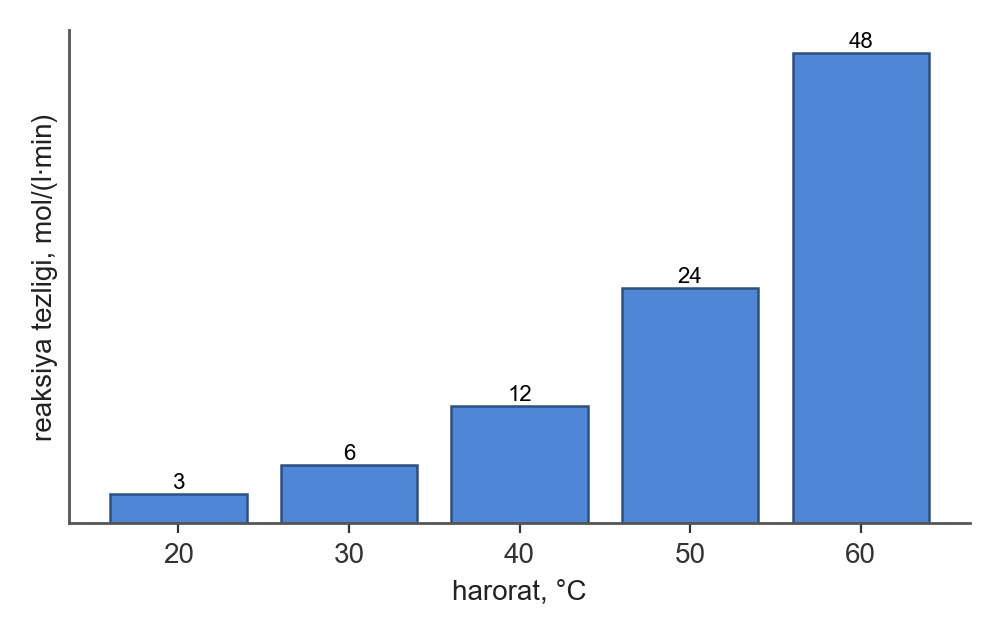
\includegraphics[width=0.86\linewidth]{rasmlar/gen/vh_v13_0.png}\end{center}
Haroratni 20 \textdegree{}C dan 50 \textdegree{}C gacha ko`tarilganda tezlik necha marta ortadi?

\noindent A)~\textsl{6} \hfill B)~\textsl{8} \hfill C)~\textsl{16} \hfill D)~\textsl{4}\par
\qsep
\noindent\qn{8.} 10 g metall kislotada eritilganda 5,6 l (n.sh.) vodorod ajraldi. Metallning ekvivalent \textbf{massasini (g/mol) aniqlang} (\textit{V}\_E(H\textsubscript{2}) = 11,2 l/mol).

\noindent A)~\textsl{20} \hfill B)~\textsl{40} \hfill C)~\textsl{10} \hfill D)~\textsl{112}\par
\qsep
\noindent\qn{9.} Li elementi ikki izotopdan iborat (massa sonlari 6 va 7). O`rtacha nisbiy atom massasi 6,9 bo`lsa, 20 g namunadagi og`ir izotopning \textbf{massasini (g) aniqlang.}

\noindent A)~\textsl{18,26} \hfill B)~\textsl{18} \hfill C)~\textsl{2} \hfill D)~\textsl{21}\par
\qsep
\noindent\qn{10.} NH\textsubscript{3} va CO aralashmasi tarkibida CO ning massasi NH\textsubscript{3} ning massasidan 6,1 g ga ko`p. Aralashmaning massasi 16,3 g. Aralashmadagi NH\textsubscript{3} ning \textbf{massasini (g) toping.}

\noindent A)~\textsl{11,2} \hfill B)~\textsl{5,1} \hfill C)~\textsl{10,2} \hfill D)~\textsl{8,15}\par
\qsep
\noindent\qn{11.} Gazlar aralashmasi tarkibi jadvalda berilgan (n.sh.):
\begin{center}
\renewcommand{\arraystretch}{1.15}
\fitbox{\begin{tabular}{|c|c|}\hline
\textbf{Gaz} & \textbf{Hajmi, l} \\ \hline
NH\textsubscript{3} & 3 \\ \hline
O\textsubscript{2} & 1 \\ \hline
He & 1 \\ \hline
\end{tabular}}
\end{center}
Aralashmaning havoga nisbatan \textbf{zichligini aniqlang} (M(havo) = 29 g/mol).

\noindent A)~\textsl{1,2} \hfill B)~\textsl{0,6} \hfill C)~\textsl{0,3} \hfill D)~\textsl{17,4}\par
\qsep
\noindent\qn{12.} Gazlar aralashmasi tarkibi jadvalda berilgan (n.sh.):
\begin{center}
\renewcommand{\arraystretch}{1.15}
\fitbox{\begin{tabular}{|c|c|}\hline
\textbf{Gaz} & \textbf{Hajmi, l} \\ \hline
He & 1 \\ \hline
Cl\textsubscript{2} & 2 \\ \hline
N\textsubscript{2} & 1 \\ \hline
\end{tabular}}
\end{center}
Aralashmaning havoga nisbatan \textbf{zichligini aniqlang} (M(havo) = 29 g/mol).

\noindent A)~\textsl{3} \hfill B)~\textsl{0,75} \hfill C)~\textsl{43,5} \hfill D)~\textsl{1,5}\par
\qsep
\noindent\qn{13.} NaCl eritmasi inert elektrodlar bilan 10 A tok kuchi bilan 3860 s elektroliz qilindi. Ajralgan gazlar aralashmasi yondirilib, hosil bo`lgan gaz 200 g suvda eritildi. Aralashmaning zichligi 2,3 g/sm\textsuperscript{3} ga teng. Olingan kislota eritmasining massa \textbf{ulushini (\%) aniqlang.}

\noindent A)~\textsl{3,52} \hfill B)~\textsl{7,3} \hfill C)~\textsl{6,8} \hfill D)~\textsl{13,61}\par
\qsep
\noindent\qn{14.} 0,5 mol SO\textsubscript{2} 0,75 mol KOH eritmasidan o`tkazildi (reaksiya oxirigacha). Hosil bo`lgan o`rta tuz \textbf{massasini (g) toping.}

\noindent A)~\textsl{30} \hfill B)~\textsl{79} \hfill C)~\textsl{39,5} \hfill D)~\textsl{19,8}\par
\qsep
\noindent\qn{15.} Probirkalardagi eritmalar: Na\textsubscript{2}SO\textsubscript{4}, Na\textsubscript{2}CO\textsubscript{3}, NaCl ni alohida probirkalarda ajratish uchun qaysi reagent(lar) yetarli? 1) BaCl\textsubscript{2} va lakmus; 2) BaCl\textsubscript{2} va fenolftalein; 3) lakmus; 4) HCl va lakmus

\noindent A)~\textsl{1, 3, 4} \hfill B)~\textsl{1} \hfill C)~\textsl{1, 2} \hfill D)~\textsl{2, 4}\par
\qsep
\noindent\qn{16.} Ishqoriy metallar haqida qaysi fikrlar to`g`ri? 1) Natriy suv bilan reaksiyada H\textsubscript{2} va NaOH hosil qiladi; 2) Natriy yonganda Na\textsubscript{2}O\textsubscript{2} hosil bo`ladi; 3) Natriyning olinishi suyuqlanma NaCl elektrolizi bilan; 4) Natriy atomining tashqi qavatida 2 ta elektron bor

\noindent A)~\textsl{1, 3} \hfill B)~\textsl{1, 2, 3} \hfill C)~\textsl{1, 4} \hfill D)~\textsl{1, 2}\par
\qsep
\noindent\qn{17.} Quyidagi jarayonlar qanday kuzatuvlar bilan boradi? To`g`ri ta'riflangan \textbf{jarayonlarni belgilang.} 1) AgNO\textsubscript{3} eritmasiga avval NaCl, so`ng mo`l ammiak eritmasi qo`shilganda: oq tvorogsimon cho`kma tushadi, keyin cho`kma sariq tusga kiradi; 2) AlCl\textsubscript{3} eritmasiga avval oz, so`ng mo`l NaOH eritmasi qo`shilganda: oq cho`kma tushadi, keyin cho`kma erib ketadi; 3) NaOH eritmasiga CuSO\textsubscript{4} eritmasi tomchilab qo`shilganda (ishqor mo`l): ko`k cho`kma tushadi, keyin ko`k cho`kma hosil bo`ladi va erimaydi; 4) FeCl\textsubscript{3} eritmasiga avval NaOH, so`ng mo`l HCl eritmasi qo`shilganda: qo`ng`ir-qizil cho`kma tushadi, keyin cho`kma erib, sariq eritma hosil bo`ladi

\noindent A)~\textsl{1, 4} \hfill B)~\textsl{1, 2} \hfill C)~\textsl{2, 3, 4} \hfill D)~\textsl{1, 3, 4}\par
\qsep
\noindent\qn{18.} Alyuminiy (0,2 mol) va kalsiy (0,2 mol) aralashmasi mo`l xlorid kislotada eritildi. Reagent (xlorid kislota) eritmasining massa ulushi 20\% va zichligi 1,12 g/ml; u mo`l miqdorda olingan. Ajralgan vodorodning \textbf{hajmini (l, n.sh.) aniqlang.}

\noindent A)~\textsl{8,96} \hfill B)~\textsl{22,4} \hfill C)~\textsl{5,6} \hfill D)~\textsl{11,2}\par
\qsep
\noindent\qn{19.} CaCO\textsubscript{3} va MgCO\textsubscript{3} aralashmasi (43,6 g) mo`l xlorid kislota bilan ta'sirlashganda 11,2 l (n.sh.) gaz ajraldi. Aralashmadagi CaCO\textsubscript{3} \textbf{massasini (g) toping.}

\noindent A)~\textsl{33,6} \hfill B)~\textsl{20} \hfill C)~\textsl{21,8} \hfill D)~\textsl{10}\par
\qsep
\noindent\qn{20.} Arenlar, neft va tabiiy gaz haqida qaysi fikrlar to`g`ri? 1) Toluol KMnO\textsubscript{4} bilan benzoy kislotagacha oksidlanadi; 2) Benzol uchun birikish reaksiyalari mutlaqo xos emas; 3) Tabiiy gazning asosiy qismi propan; 4) Naftalin -- bir halqali aren

\noindent A)~\textsl{2, 3} \hfill B)~\textsl{3, 4} \hfill C)~\textsl{1} \hfill D)~\textsl{2}\par
\qsep
\noindent\qn{21.} Murakkab efirlar va yog`lar haqida qaysi fikrlar to`g`ri? 1) Efirlanish reaksiyasi qaytmas; 2) Murakkab efirlarning gidrolizi ishqoriy muhitda qaytmas; 3) Suyuq yog`lar to`yinmagan kislotalardan hosil bo`lgan; 4) Etilatsetat efir hidli suyuqlik

\noindent A)~\textsl{1, 3, 4} \hfill B)~\textsl{1, 4} \hfill C)~\textsl{2, 3, 4} \hfill D)~\textsl{2, 4}\par
\qsep
\noindent\qn{22.} Quyidagi birikmalardan qaysi biri murakkab efir sinfiga kiradi?

\noindent\begin{tabular}{@{}p{0.47\linewidth}@{}p{0.47\linewidth}@{}}
A)~\textsl{C\textsubscript{2}H\textsubscript{5}NH\textsubscript{2}} & B)~\textsl{C\textsubscript{12}H\textsubscript{22}O\textsubscript{11}} \\
C)~\textsl{C\textsubscript{2}H\textsubscript{5}OH} & D)~\textsl{CH\textsubscript{3}COOC\textsubscript{2}H\textsubscript{5}} \\
\end{tabular}\par
\qsep
\noindent\qn{23.} Etilen va vodorod aralashmasi (mol nisbati 2 : 5) Ni katalizatori ustida to`liq gidrogenlandi. Reaksiyadan so`ng hosil bo`lgan gazlar aralashmasining vodorodga nisbatan \textbf{zichligini aniqlang.}

\noindent A)~\textsl{4,7} \hfill B)~\textsl{13,2} \hfill C)~\textsl{3,3} \hfill D)~\textsl{6,6}\par
\qsep
\noindent\qn{24.} Rasmda tasvirlangan molekuladagi sp\textsuperscript{3}-gibridlangan uglerod atomlari \textbf{sonini aniqlang.}
\begin{center}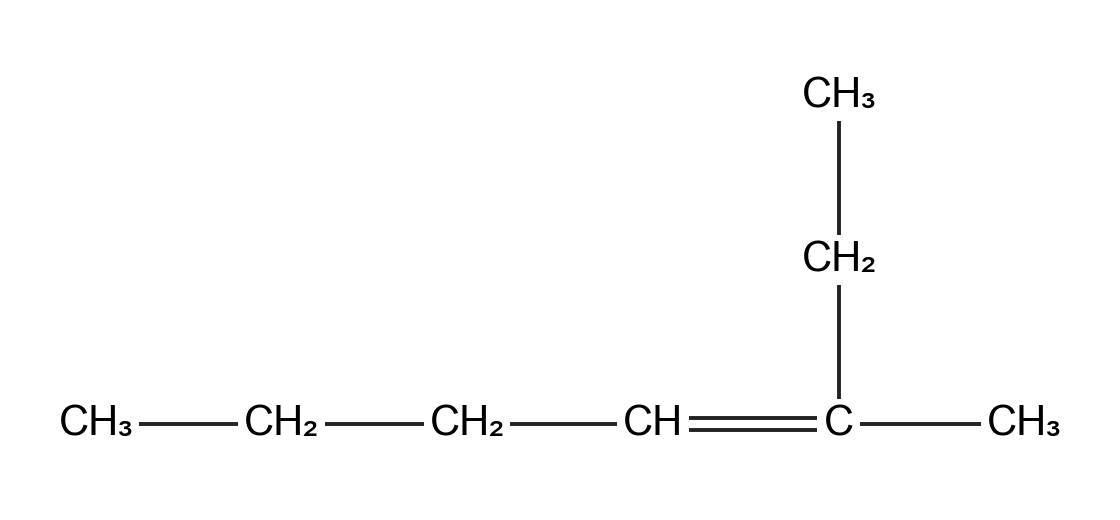
\includegraphics[width=0.86\linewidth]{rasmlar/gen/struct_16944700_887.png}\end{center}

\noindent A)~\textsl{6} \hfill B)~\textsl{7} \hfill C)~\textsl{5} \hfill D)~\textsl{8}\par
\qsep
\noindent\qn{25.} C\textsubscript{2}H\textsubscript{2} va CH\textsubscript{4} aralashmasi tarkibida aralashmadagi vodorod atomlari sonining uglerod atomlari soniga nisbati 3 : 2. Shu aralashmani yondirish uchun 36,96 l (n.sh.) kislorod sarflandi. Aralashmadagi C\textsubscript{2}H\textsubscript{2} ning \textbf{massasini (g) toping.}

\noindent A)~\textsl{3,2} \hfill B)~\textsl{26} \hfill C)~\textsl{8,1} \hfill D)~\textsl{13}\par
\qsep
\noindent\qn{26.} 64 g texnik CaC\textsubscript{2} (tarkibida 75\% sof modda) dan quyidagi sxema bo`yicha 27,09 g polivinilxlorid olindi: CaC\textsubscript{2} $\to$ C\textsubscript{2}H\textsubscript{2} $\to$ CH\textsubscript{2}=CHCl $\to$ (--CH\textsubscript{2}--CHCl--)n. Dastlabki 2 bosqichning unumi ketma-ket 85\%, 80\% ga teng. Barcha reaksiyalar 1,5 atm bosimda olib borildi. Oxirgi bosqichning \textbf{unumini (\%) aniqlang.}

\noindent A)~\textsl{42} \hfill B)~\textsl{85} \hfill C)~\textsl{15} \hfill D)~\textsl{68}\par
\qsep
\noindent\qn{27.} 120 g CH\textsubscript{3}COOH dan quyidagi sxema bo`yicha glitsilglitsin olindi: CH\textsubscript{3}COOH $\to$ ClCH\textsubscript{2}COOH $\to$ H\textsubscript{2}N--CH\textsubscript{2}--COOH $\to$ dipeptid. Bosqichlarning unumi ketma-ket 75\%, 80\%, 90\% ni tashkil qiladi. Barcha reaksiyalar 1,5 atm bosimda olib borildi. Olingan glitsilglitsin \textbf{massasini (g) aniqlang.}

\noindent A)~\textsl{142,56} \hfill B)~\textsl{35,64} \hfill C)~\textsl{79,2} \hfill D)~\textsl{71,28}\par
\qsep
\noindent\qn{28.} CaC\textsubscript{2} dan quyidagi sxema bo`yicha 84,46 g etanol olindi: CaC\textsubscript{2} $\to$ C\textsubscript{2}H\textsubscript{2} $\to$ C\textsubscript{2}H\textsubscript{4} $\to$ C\textsubscript{2}H\textsubscript{5}OH. Bosqichlarning unumi ketma-ket 90\%, 85\%, 60\% ni tashkil qiladi. Sarflangan CaC\textsubscript{2} massasi (g) \textbf{ni aniqlang.}

\noindent A)~\textsl{512} \hfill B)~\textsl{256} \hfill C)~\textsl{128} \hfill D)~\textsl{230,4}\par
\qsep
\noindent\qn{29.} C\textsubscript{12}H\textsubscript{22}O\textsubscript{11} dan quyidagi sxema bo`yicha 264,96 g etanol olindi: C\textsubscript{12}H\textsubscript{22}O\textsubscript{11} $\to$ C\textsubscript{6}H\textsubscript{12}O\textsubscript{6} (glyukoza va fruktoza) $\to$ C\textsubscript{2}H\textsubscript{5}OH. Bosqichlarning unumi ketma-ket 80\%, 90\% ni tashkil qiladi. Sarflangan C\textsubscript{12}H\textsubscript{22}O\textsubscript{11} massasi (g) \textbf{ni aniqlang.}

\noindent A)~\textsl{684} \hfill B)~\textsl{1368} \hfill C)~\textsl{342} \hfill D)~\textsl{547,2}\par
\qsep
\noindent\qn{30.} Raqamlangan (1--4) probirkalarda BaCl\textsubscript{2}, HCl, Na\textsubscript{2}CO\textsubscript{3}, NaOH eritmalari tartibsiz holda berilgan. Quyidagi kuzatuvlar asosida moddalarni probirka raqami bilan moslang. 2- va 3-probirkalardagi eritmalar aralashtirilganda oq cho`kma tushadi. 1- va 4-probirkalardagi eritmalar aralashtirilganda bir-birini neytrallaydi. 1- va 3-probirkalardagi eritmalar aralashtirilganda rangsiz, hidsiz gaz ajraladi.
\noindent A)~\textsl{1-HCl, 2-BaCl\textsubscript{2}, 3-Na\textsubscript{2}CO\textsubscript{3}, 4-NaOH}\par
\noindent B)~\textsl{1-HCl, 2-BaCl\textsubscript{2}, 3-NaOH, 4-Na\textsubscript{2}CO\textsubscript{3}}\par
\noindent C)~\textsl{1-BaCl\textsubscript{2}, 2-HCl, 3-Na\textsubscript{2}CO\textsubscript{3}, 4-NaOH}\par
\noindent D)~\textsl{1-NaOH, 2-BaCl\textsubscript{2}, 3-Na\textsubscript{2}CO\textsubscript{3}, 4-HCl}\par
\qsep
\noindent\qn{31.} Quyidagi jarayonlar qanday kuzatuvlar bilan boradi? To`g`ri ta'riflangan \textbf{jarayonlarni belgilang.} 1) NaOH eritmasiga CuSO\textsubscript{4} eritmasi tomchilab qo`shilganda (ishqor mo`l): ko`k cho`kma tushadi, keyin ko`k cho`kma hosil bo`ladi va erimaydi; 2) Na\textsubscript{2}CO\textsubscript{3} eritmasiga HCl eritmasi tomchilab (kislota yetishmaganda) qo`shilganda: gaz ajralmaydi (NaHCO\textsubscript{3} hosil bo`ladi), keyin kislota ko`paytirilsa, gaz ajrala boshlaydi; 3) AlCl\textsubscript{3} eritmasiga avval oz, so`ng mo`l NaOH eritmasi qo`shilganda: oq cho`kma tushadi, keyin cho`kma erimasdan qoladi; 4) ZnSO\textsubscript{4} eritmasiga avval oz, so`ng mo`l NaOH eritmasi qo`shilganda: oq cho`kma tushadi, keyin cho`kma erimasdan qoladi

\noindent A)~\textsl{1, 2, 4} \hfill B)~\textsl{1, 3} \hfill C)~\textsl{1, 3, 4} \hfill D)~\textsl{1, 2}\par
\qsep
\noindent\qn{32.} Rasmdagi usul bilan qaysi aralashmani ajratish mumkin?
\begin{center}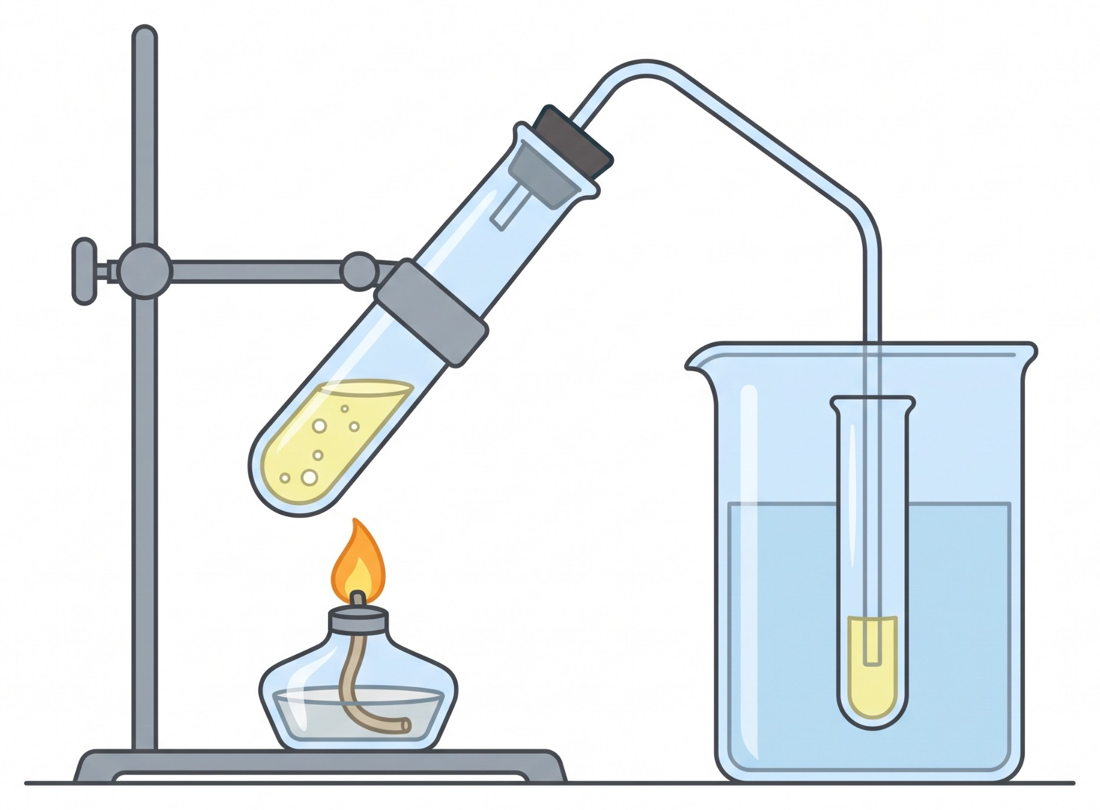
\includegraphics[width=0.86\linewidth]{rasmlar/darslik/d_distill.png}\end{center}

\noindent\begin{tabular}{@{}p{0.47\linewidth}@{}p{0.47\linewidth}@{}}
A)~\textsl{suv va etanol} & B)~\textsl{osh tuzi va qum} \\
C)~\textsl{suv va kerosin} & D)~\textsl{suv va qum   ---} \\
\end{tabular}\par
\qsep
\end{multicols}
\medskip
\noindent\setlength{\fboxsep}{0pt}\fbox{\begin{tabular}{p{0.74\linewidth}|p{0.2\linewidth}}
\parbox[t]{0.72\linewidth}{\vspace{3pt}\textbf{Topshiriqlar (33--35) va javob variant (A--F)larini o`zaro to`g`ri moslashtiring.} 18,8 g Cu(NO\textsubscript{3})\textsubscript{2} doimiy massagacha qizdirildi, ajralgan gazlar suvga yuttirilib, hajmi 2 l bo`lgan eritma tayyorlandi. Qoldiq shu eritmada to`liq eritildi (kislota qoldiqsiz sarflandi), olingan eritma (hajmi o`zgarmadi deb hisoblang) 10 A tok kuchi bilan 1544 s inert elektrodlarda elektroliz qilindi.
\vspace{3pt}} & \parbox[t]{0.19\linewidth}{\vspace{3pt}A~\textsl{0,03}\\[3pt]
B~\textsl{1}\\[3pt]
C~\textsl{0,05}\\[3pt]
D~\textsl{2}\\[3pt]
E~\textsl{0,08}\\[3pt]
F~\textsl{5,12}}\\ \hline
\parbox[t]{0.72\linewidth}{\vspace{2pt}\textbf{33. Gazlar yutilgach hosil bo`lgan eritmaning pH ini aniqlang.}\vspace{2pt}} & \\ \hline
\parbox[t]{0.72\linewidth}{\vspace{2pt}\textbf{34. Qoldiq erigandan so`ng Cu(NO\textsubscript{3})\textsubscript{2} ning molyar konsentratsiyasini (mol/l) hisoblang.}\vspace{2pt}} & \\ \hline
\parbox[t]{0.72\linewidth}{\vspace{2pt}\textbf{35. Elektrolizda katodda ajralgan metall massasini (g) toping.}\vspace{2pt}} & 
\end{tabular}}
\par\bigskip
\noindent\qn{36.} 40\% li va 20\% li tuz eritmalari massalar nisbati 1 : 3 bo`lgan holda aralashtirildi. Tajriba laboratoriyada, chinni idishda o`tkazildi. Hosil bo`lgan eritmaning massa \textbf{ulushini (\%) hisoblang.}
\javob\qsep
\noindent\qn{37.} AgNO\textsubscript{3} eritmasi inert elektrodlar yordamida 4 A tok kuchi bilan 9650 s elektroliz qilindi. Elektrolizyorning hajmi 3 l. Katodda ajralgan Ag massasi (g) \textbf{ni toping.}
\javob\qsep
\noindent\qn{38.} 2SO\textsubscript{3} $\rightleftarrows$ 2SO\textsubscript{2} + O\textsubscript{2} reaksiyasi doimiy harorat va bosimda olib borildi; boshlang`ich modda qisman o`zgargach gazlar hajmi 9/8 marta ortdi. Tajriba 40 daqiqa davom etdi. Boshlang`ich modda necha foizi \textbf{o`zgarganini aniqlang.}
\javob\qsep
\noindent\qn{39.} 49,2 g nitrobenzol qaytarilib anilin olindi (unum 3/4). Hosil bo`lgan anilinning 1/2 qismi mo`l bromli suv bilan ta'sirlashtirildi. Barcha reaksiyalar 1,5 atm bosimda olib borildi. Hosil bo`lgan cho`kmaning \textbf{massasini (g) toping.}
\javob\qsep
\noindent\qn{40.} 11,2 l (n.sh.) atsetilen Kucherov reaksiyasi bo`yicha gidratlandi (unum 4/5); hosil bo`lgan aldegidning 2/5 qismi ammiakli kumush oksid eritmasi bilan qizdirildi. Barcha reaksiyalar 1 atm bosimda olib borildi. Ajralgan kumush \textbf{massasini (g) hisoblang.}
\javob\qsep
\par\bigskip\begin{center}\textbf{\fontsize{13}{15}\selectfont YOZMA ISH}\end{center}
\noindent\qn{41.} \textbf{Topshiriqni bajarish jarayonida barcha reaksiya tenglamalarini yozing. Miqdoriy va arifmetik hisoblashlarni (unga asos bo`lgan usul yoki formulani ko`rsatgan holda) uzviy ketma-ketlikda bajaring.}\par\smallskip
Cu(NO\textsubscript{3})\textsubscript{2} va NaNO\textsubscript{3} dan iborat 54,5 g aralashma doimiy massagacha qizdirildi. Ajralgan gazlar aralashmasi sovitilib, 300 g suvga yuborildi Qattiq qoldiq suvga tushirilganda NaNO\textsubscript{2} erib, CuO erimay qoldi; cho`kma ajratilib, 10\% li sulfat kislotaning stexiometrik miqdorida eritildi. Elektrolizyorning hajmi 5 l. Hosil bo`lgan eritma inert elektrodlar yordamida 10 A tok kuchi bilan 3088 s elektroliz qilindi (Cu\textsuperscript{2+} ning bir qismi eritmada qoldi).\par
\noindent 1)\ Barcha jarayonlarning reaksiya tenglamalarini yozing va tenglashtiring. Qizdirishda ajralgan gazlarning mol miqdorlarini va yutilmay qolgan gaz hajmini (l, n.sh.) hisoblang.\par
\noindent 2)\ Gazlar yutilgandan keyingi eritmada HNO\textsubscript{3} ning massa ulushini (\%) toping. Qattiq qoldiqdagi NaNO\textsubscript{2} va CuO massalarini (g) aniqlang.\par
\noindent 3)\ CuO sulfat kislotada erigandan keyingi eritmada CuSO\textsubscript{4} ning massa ulushini (\%) hisoblang.\par
\noindent 4)\ Elektrolizda katodda ajralgan mis massasini (g) va anodda ajralgan gaz hajmini (l, n.sh.) toping.\par
\noindent 5)\ Elektroliz tugagach eritmadagi CuSO\textsubscript{4} va H\textsubscript{2}SO\textsubscript{4} ning massa ulushlarini (\%) aniqlang.\par
\diqqat{Mazkur topshiriq kengaytirilgan javobni talab etib, uning yechilish usuli va shu usul asosidagi barcha hisoblash amallari javoblar varaqasida aks etishi lozim.}\qsep
\noindent\qn{42.} Organik moddalarning xossalarini bilgan holda reaksiya tenglamalarini tugallang va tenglashtiring. 3- va 5-reaksiyalarda hosil bo`lgan asosiy organik mahsulotlarni sistematik nomenklatura bo`yicha nomlang. Hosil bo`lgan organik moddalarning tuzilish formulalarini yozing.\par
\noindent 1)\ CH\textsubscript{3}--CHCl--CH\textsubscript{3} + KOH (spirtli eritma, t) $\to$\par
\noindent 2)\ CH\textsubscript{2}=CH--CH=CH\textsubscript{2} + Br\textsubscript{2} (1 : 1, 1,4-birikish) $\to$\par
\noindent 3)\ C\textsubscript{6}H\textsubscript{5}--NH\textsubscript{2} + Br\textsubscript{2} (suvli eritma) $\to$\par
\noindent 4)\ H\textsubscript{2}N--CH\textsubscript{2}--COOH + NaOH $\to$\par
\noindent 5)\ CH\textsubscript{3}--CH\textsubscript{2}--CH(OH)--CH\textsubscript{3} (H\textsubscript{2}SO\textsubscript{4} kons., t) $\to$\par
\noindent 6)\ CH\textsubscript{3}--CHO + H\textsubscript{2} (Ni, t) $\to$\par
\noindent 7)\ CH\textsubscript{3}--COOH + Cl\textsubscript{2} (P, t) $\to$\par
\diqqat{Mazkur topshiriq kengaytirilgan javobni talab etib, uning yechilish usuli va shu usul asosidagi barcha hisoblash amallari javoblar varaqasida aks etishi lozim.}\qsep
\noindent\qn{43.} \textbf{Topshiriqni bajarish jarayonida barcha reaksiya tenglamalarini yozing. Miqdoriy va arifmetik hisoblashlarni (unga asos bo`lgan usul yoki formulani ko`rsatgan holda) uzviy ketma-ketlikda bajaring.}\par\smallskip
CaCO\textsubscript{3} va MgCO\textsubscript{3} dan iborat aralashmada ularning massalari nisbati 25 : 21. Aralashma doimiy massagacha qizdirilganda massasi 17,6 g ga kamaydi. Ajralgan gaz 0,5 mol NaOH saqlagan eritmaga yuttirildi (gaz to`liq yutildi), hosil bo`lgan eritmaga mo`l BaCl\textsubscript{2} eritmasi qo`shildi. Qizdirishdan qolgan qattiq qoldiq esa 10\% li xlorid kislotaning stexiometrik miqdorida eritildi. Qizdirish 60 daqiqa davom etdi. Qoldiqning HCl dagi eritmasiga mo`l Na\textsubscript{2}CO\textsubscript{3} eritmasi qo`shilib, hosil bo`lgan cho`kma ajratildi va doimiy massagacha qizdirildi; ajralgan gaz mo`l ohakli suvga yuborildi.\par
\noindent 1)\ Barcha reaksiyalarning tenglamalarini yozing va tenglashtiring. Dastlabki aralashmadagi karbonatlarning massalarini (g) aniqlang.\par
\noindent 2)\ Ajralgan gazning hajmini (l, n.sh.) hisoblang va hosil bo`lgan tuzlar tarkibini (o`rta/nordon) aniqlang.\par
\noindent 3)\ Gaz yutilgandan keyingi eritmadagi tuzlarning massalarini (g) toping. Na\textsubscript{2}CO\textsubscript{3} qo`shilganda hosil bo`lgan cho`kmalarning umumiy massasini (g) hisoblang.\par
\noindent 4)\ BaCl\textsubscript{2} qo`shilganda hosil bo`lgan cho`kma massasini (g) hisoblang. Cho`kma qizdirilganda massa necha gramga kamayadi?\par
\noindent 5)\ Qoldiq erigan eritmaning massasini (g) va undagi tuzlarning massa ulushlarini (\%) toping. Ohakli suvga yuborilganda hosil bo`lgan cho`kma massasini (g) toping.\par
\diqqat{Mazkur topshiriq kengaytirilgan javobni talab etib, uning yechilish usuli va shu usul asosidagi barcha hisoblash amallari javoblar varaqasida aks etishi lozim.}\qsep
\newpage
\noindent\textbf{\fontsize{13}{15}\selectfont 13-variant}\hfill \textbf{Javoblar kaliti}\par\smallskip\hrule\smallskip
\textit{Faqat o`qituvchi uchun.}\par\medskip
\noindent\textbf{1--32-savollar}\par\smallskip
\noindent\begin{tabular}{|c|c|c|c|c|c|c|c|c|c|c|c|c|c|c|c|}\hline
\textbf{1} & \textbf{2} & \textbf{3} & \textbf{4} & \textbf{5} & \textbf{6} & \textbf{7} & \textbf{8} & \textbf{9} & \textbf{10} & \textbf{11} & \textbf{12} & \textbf{13} & \textbf{14} & \textbf{15} & \textbf{16}\\\hline
\textsl{A} & \textsl{A} & \textsl{C} & \textsl{C} & \textsl{B} & \textsl{B} & \textsl{B} & \textsl{A} & \textsl{A} & \textsl{B} & \textsl{B} & \textsl{D} & \textsl{C} & \textsl{C} & \textsl{C} & \textsl{B}\\\hline
\textbf{17} & \textbf{18} & \textbf{19} & \textbf{20} & \textbf{21} & \textbf{22} & \textbf{23} & \textbf{24} & \textbf{25} & \textbf{26} & \textbf{27} & \textbf{28} & \textbf{29} & \textbf{30} & \textbf{31} & \textbf{32}\\\hline
\textsl{C} & \textsl{D} & \textsl{D} & \textsl{C} & \textsl{C} & \textsl{D} & \textsl{D} & \textsl{A} & \textsl{D} & \textsl{B} & \textsl{D} & \textsl{B} & \textsl{A} & \textsl{A} & \textsl{D} & \textsl{A}\\\hline
\end{tabular}\par\medskip
\noindent\textbf{33--35-savollar}\par\smallskip
\noindent\begin{tabular}{|c|c|c|}\hline \textbf{No} & \textbf{Javob} & \textbf{Qiymat}\\\hline
33 & \textsl{B} & 1\\\hline
34 & \textsl{C} & 0,05\\\hline
35 & \textsl{F} & 5,12\\\hline
\end{tabular}\par\medskip
\noindent\textbf{36--40-savollar}\par\smallskip
\noindent\begin{tabular}{|c|c|}\hline \textbf{No} & \textbf{To`g`ri javob}\\\hline
36 & 25\\\hline
37 & 43,2\\\hline
38 & 25\\\hline
39 & 49,5\\\hline
40 & 34,56\\\hline
\end{tabular}\par\medskip
\noindent\textbf{41--43-topshiriqlar: javoblar}\par\smallskip
\noindent\textbf{41-topshiriq.}\par
\noindent 1) 0,4 mol; 0,2 mol; 2,24 l\par
\noindent 2) 7,84\%; 16 g; 13,8 g\par
\noindent 3) 15,09\%\par
\noindent 4) 10,24 g; 1,79 l\par
\noindent 5) 3,21\%; 7,87\%\par
\noindent\textbf{42-topshiriq.}\par
\noindent 1) CH\textsubscript{3}--CHCl--CH\textsubscript{3} + KOH $\to$ CH\textsubscript{3}--CH=CH\textsubscript{2} + KCl + H\textsubscript{2}O\par
\noindent 2) CH\textsubscript{2}=CH--CH=CH\textsubscript{2} + Br\textsubscript{2} $\to$ BrCH\textsubscript{2}--CH=CH--CH\textsubscript{2}Br\par
\noindent 3) C\textsubscript{6}H\textsubscript{5}--NH\textsubscript{2} + 3Br\textsubscript{2} $\to$ C\textsubscript{6}H\textsubscript{2}Br\textsubscript{3}--NH\textsubscript{2}$\downarrow$ + 3HBr --- nomi: \textbf{2,4,6-tribromanilin}\par
\noindent 4) H\textsubscript{2}N--CH\textsubscript{2}--COOH + NaOH $\to$ H\textsubscript{2}N--CH\textsubscript{2}--COONa + H\textsubscript{2}O\par
\noindent 5) CH\textsubscript{3}--CH\textsubscript{2}--CH(OH)--CH\textsubscript{3} $\to$ CH\textsubscript{3}--CH=CH--CH\textsubscript{3} + H\textsubscript{2}O (Zaysev qoidasi) --- nomi: \textbf{buten-2}\par
\noindent 6) CH\textsubscript{3}--CHO + H\textsubscript{2} $\to$ CH\textsubscript{3}--CH\textsubscript{2}--OH\par
\noindent 7) CH\textsubscript{3}--COOH + Cl\textsubscript{2} $\to$ CH\textsubscript{2}Cl--COOH + HCl\par
\noindent\textbf{43-topshiriq.}\par
\noindent 1) 20 g; 16,8 g\par
\noindent 2) 8,96 l\par
\noindent 3) 10,6 g; 25,2 g; 36,8 g\par
\noindent 4) 19,7 g; 17,6 g\par
\noindent 5) 311,2 g; 7,13\%; 6,11\%; 40 g\par
\par\bigskip\noindent\textbf{Mavzular taqsimoti}\par\smallskip
{\small\noindent\begin{longtable}{|c|p{7.2cm}|p{5.4cm}|c|}\hline \textbf{No} & \textbf{Mavzu} & \textbf{Tekshiriladigan ko`nikma} & \textbf{Ball}\\\hline
1 & Tashev; 9-sinf (kuchlanish qatori) & Bilim va tushunish & 1\\\hline
2 & 11-sinf 8-bob; Tirkashev \textit{V} bob (elektroliz) & Bilim va tushunish & 1\\\hline
3 & 9-sinf; 11-sinf (tuzlar gidrolizi; Le-Shatelye) & Bilim va tushunish & 1\\\hline
4 & 11-sinf 4-bob (molyar konsentratsiya) & Hisoblash va masala yechish & 1\\\hline
5 & 8-sinf; Tirkashev II bob (kimyoviy bog`lanish) & Bilim va tushunish & 1\\\hline
6 & 11-sinf 8-bob; Tirkashev \textit{V} bob (elektroliz) & Bilim va tushunish & 1\\\hline
7 & Tirkashev VI bob (Vant-Goff qoidasi, grafik) & Grafik tahlili & 1\\\hline
8 & 11-sinf (ekvivalentlar qonuni) & Hisoblash va masala yechish & 1\\\hline
9 & 8-sinf (izotoplar; o`rtacha atom massa) & Hisoblash va masala yechish & 1\\\hline
10 & 8-9-sinf (gaz aralashmalari; Avogadro qonuni) & Hisoblash va masala yechish & 1\\\hline
11 & 11-sinf (gaz aralashmalar, jadval) & Jadval tahlili & 1\\\hline
12 & 11-sinf (gaz aralashmalar, jadval) & Jadval tahlili & 1\\\hline
13 & 9-sinf; 11-sinf (elektroliz; vodorod xlorid) & Hisoblash va masala yechish & 1\\\hline
14 & 9-sinf (kislotali oksidlarning ishqor bilan reaksiyasi) & Hisoblash va masala yechish & 1\\\hline
15 & 9-sinf (ion reaksiyalar, anionlarni aniqlash) & Bilim va tushunish & 1\\\hline
16 & 9-sinf (ishqoriy metallar); Tashev & Bilim va tushunish & 1\\\hline
17 & 9-sinf; 11-sinf (amfoter birikmalar, kompleks hosil bo`lishi) & Bilim va tushunish & 1\\\hline
18 & 9-sinf & Hisoblash va masala yechish & 1\\\hline
19 & 8-9-sinf (karbonatlar; kislotalar bilan reaksiya) & Hisoblash va masala yechish & 1\\\hline
20 & 10-sinf (mavzuga oid paragraflar); Abdusamatov & Bilim va tushunish & 1\\\hline
21 & 10-sinf (mavzuga oid paragraflar); Abdusamatov & Bilim va tushunish & 1\\\hline
22 & 10-sinf (organik birikmalar sinflari) & Bilim va tushunish & 1\\\hline
23 & 10-sinf (alkenlarni gidrogenlash) & Hisoblash va masala yechish & 1\\\hline
24 & 10-sinf (gibridlanish) & Rasm bo`yicha tahlil & 1\\\hline
25 & 10-sinf (uglevodorodlarning yonishi) & Hisoblash va masala yechish & 1\\\hline
26 & 10-sinf (polimerlar; vinilxlorid olinishi) & Hisoblash va masala yechish & 1\\\hline
27 & 10-sinf (aminokislotalar, peptidlar) & Hisoblash va masala yechish & 1\\\hline
28 & 10-sinf (alkinlar, alkenlar, spirtlar) & Hisoblash va masala yechish & 1\\\hline
29 & 10-sinf (disaxaridlar; bijg`ish) & Hisoblash va masala yechish & 1\\\hline
30 & 9-sinf; 10-sinf (sifat reaksiyalari, ion almashinish) & Bilim va tushunish & 1\\\hline
31 & 9-sinf; 11-sinf (amfoter birikmalar, kompleks hosil bo`lishi) & Bilim va tushunish & 1\\\hline
32 & 7-sinf (13-rasm) & Rasm bo`yicha tahlil & 1\\\hline
33--35 & Aralash masala (moslashtirish) & Ko`p bosqichli hisob & 3\\\hline
36--40 & Qisqa javobli masalalar & Hisoblash & 5\\\hline
41--43 & Yozma ish & Usul va hisob (M, A) & 75\\\hline
\end{longtable}}
\end{document}
